\begin{homeworkProblem}

\textbf{Binary Sequences with No Adjacent 1s:} compute the expected number of $1$s in a good sequence if all good sequences are equal likely ($m=150$)

(a) Find the analytical solution

(b) Implement a DTMC based MCMC algorithm for approximate computing

(c) Implement a CTMC based MCMC algorithm for approximate computing

\solution

(a) This can be modeled as a dynamic programming problem. Let $f_n$ donotes the number of good sequences whose length is $n$, and $g_n$ donates the number of $1$s among all good sequences whose length is $n$. Then for the border case, we can obviously get that $f_0=1, f_1=2, g_0=0, g_1=1$. And for $n\geq 2$, we can consider $2$ cases: \\
1. If a good sequence with length $n$, ends with $0$, then the $(n-1)$-th bit can be $0$ or $1$. And these sequences has number of $f_{n-1}$, contributes $g_{n-1}$ 1s to the total number of 1s. \\
2. If a good sequence with length $n$, ends with $1$, then the $(n-1)$-th bit must be $0$, which is the same meaning that the $n-2$-th bit can be $0$ or $1$. And these sequences has number of $f_{n-2}$, contributes $g_{n-2}+f_{n-2}$ 1s to the total number of 1s.\\
So above all, we can get the recursive equation:
\begin{align*}
f_n &= f_{n-1} + f_{n-2} \qquad\qquad\ ,n\geq 2 \\
g_n &= g_{n-1} + g_{n-2} + f_{n-2} \quad ,n\geq 2
\end{align*}
We can compute the $f_m$ and $g_m$ to get the analytical solution. Since there are total $f_m$ good sequences, and $g_m$ total number of 1s, so the expectede number of 1s in a godd sequence is $\dfrac{g_m}{f_m}$.
\\
The analytical solution of $m = 150$ is $41.6117667420032$.

(b) We can design a Markov Chain. Each state $X$ is a good sequence with length $m$. For each transition, we uniformly choose one of its $m$ components, and flip that bit to generate a new state. If the new state is a good sequence, then translate to the new state, otherwise translate to the old state itself. An example of $m=4$ is as follows:
\begin{figure}[h]
    \centering
    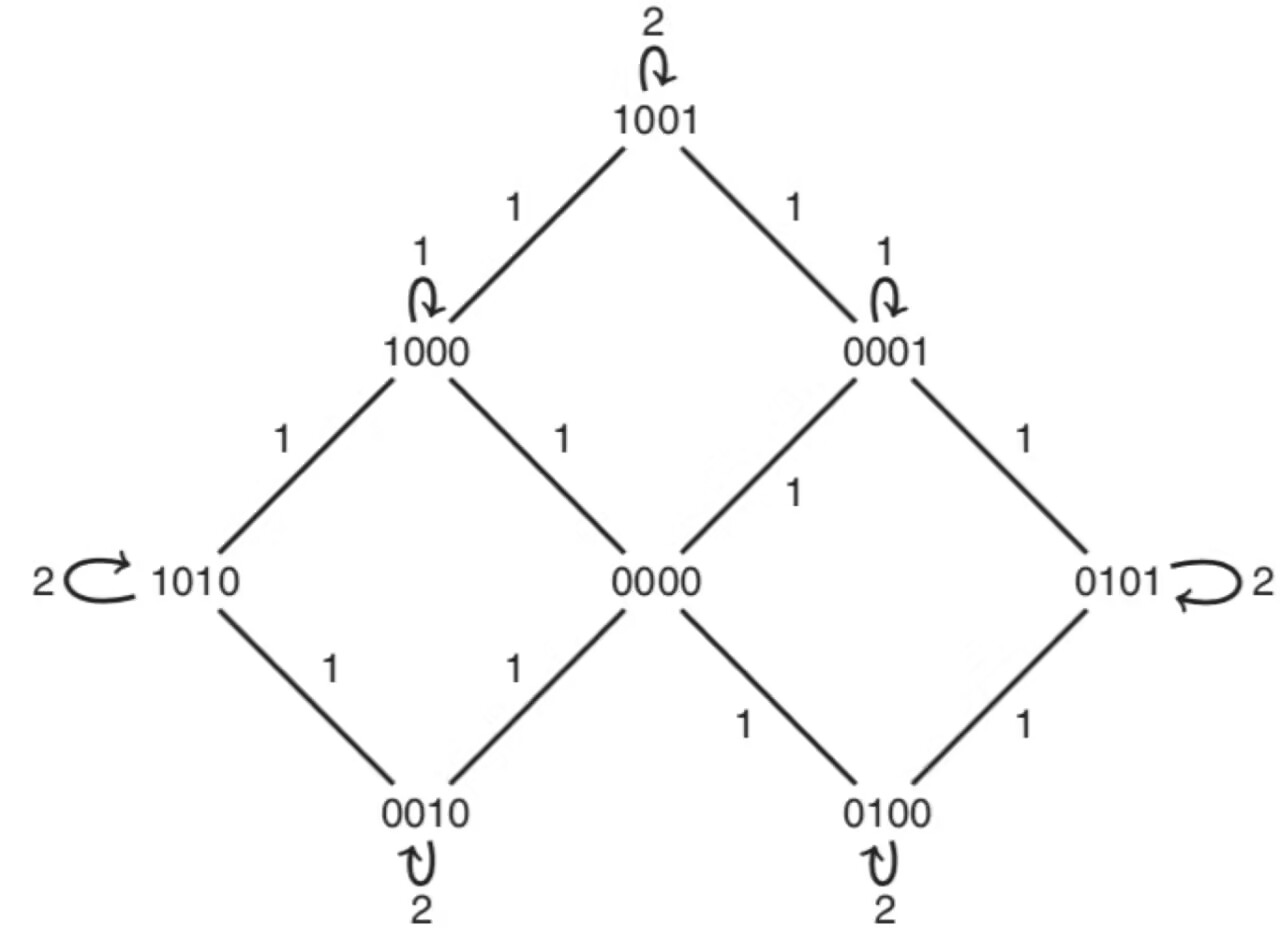
\includegraphics[width=0.5\textwidth]{./figure/p1/chain.png}
\end{figure}

1. Finite state: Since the number of good sequence with length $m$ would not exceed $2^m$, so the Markov Chain is finite state. \\
2. Irreducible: Since for each state $X$, it requires at most $m$ steps to translate to the state that is all $0$. So for any two state in the Markov Chain requires at most $2m$ step to translate to each other, so the Markov Chain is irreducible. \\
3. Aperiodic: Since for the good sequences with at least one $1$, it must have a transition to itself if $m>1$, so the Markov Chain is aperiodic. \\
So the Markov Chain is finite state, irreducible and aperiodic, which means it's ergodic, so it has a unique stationary distribution.

Since for two state $i,j$, if the Hamming distance between $i$ and $b$ is $j$, then $p_{i,j}=p_{j,i}=\dfrac{1}{m}$, and otherwise $p_{i,j}=p_{j,i}=0$. So the transition matrix is symmetric, which means it is a double stochastic matrix. So the unique stationary distribution is the uniform distribution, which is exactly what we want.

Define $r(X)$ be the number of $1$s for the state $X$. From the Strong Law of Large Numbers for Markov Chains, we have
$$\E\left[r(X)\right] = \lim_{n\to\infty}\dfrac{r(X_1)+\ldots+r(X_n)}{n}$$
So we can simulate by calculating the right hand size and get the expected number of 1s in a good sequence. \\
The simulated approximated solution using DTMC based MCMC of $m = 150$ is $41.606899$. Which is quite close to the analytical solution.

(c) Similarly with the construction in (b), but the time becomes continuous. Consider the state $i$, let $\N_i$ be the neighbors of state $i$, which means if state $j\in\N_i$, then the Hamming distance between state $i$ and state $j$ is $1$, and state $j$ is a good sequence. Then the transiton probability of the embedded chain is $p_{i,j}^e=\dfrac{1}{|\N_i|}$. \\
From the detailed balance equation: $\forall i,j$, we have
$$\pi_i q_{i,j}=\pi_j q_{j,i}$$
Since we want the stationary distribution to be a uniform distribution, and $q_{i,j}=p_{i,j}^ev_i$, thus we need to set the holding time of state $i$ to be $T_i\sim\Expo(|\N_i|)$. \\
To simulate the CTMC based MCMC, we can easily apply the Gillespie algorithm. Suppose the state transition occurs at time $0=t_0< t_1<\ldots<t_N=T$, then we can expand the Strong Law of Large Numbers for Markov Chains to be:
$$\E\left[r(X)\right]=\lim_{T\to+\infty}\int_{0}^T\dfrac{r(X_t)}{T}\dt=\lim_{N\to\infty}\sum_{n=1}^N\dfrac{r(X_{t_n})\cdot(t_n-t_{n-1})}{T}$$
The simulated approximated solution using CTMC based MCMC of $m = 150$ is $41.59466945403054$. Which is quite close to the analytical solution. And we can see that both DTMC and CTMC based MCMC have the similar results, both quite close to the analytical solution. But CTMC cost more times compared to DTMC in the same steps. This is because CTMS need to get all the neigbors of the state, which requires additionally $O(m)$ time.

\end{homeworkProblem}

\newpage